\documentclass[conference]{IEEEtran}
\IEEEoverridecommandlockouts
% The preceding line is only needed to identify funding in the first footnote. If that is unneeded, please comment it out.
\usepackage[british,UKenglish,USenglish,english,american]{babel}

\usepackage{cite}
\usepackage{float}
\usepackage{amsmath,amssymb,amsfonts}
\usepackage{algorithmic}
\usepackage{graphicx}
\usepackage{textcomp}
\usepackage{xcolor}
\def\BibTeX{{\rm B\kern-.05em{\sc i\kern-.025em b}\kern-.08em
    T\kern-.1667em\lower.7ex\hbox{E}\kern-.125emX}}
\begin{document}

\title{Optimization of dynamic routing, space and spectrum allocation
(RSSA) of unicast demands in flex-grid network\\
{\footnotesize \textsuperscript{} Zaawansowane metody projektowania sieci teleinformatycznych}
}

\author{\IEEEauthorblockN{Maciej Bakowicz}
\IEEEauthorblockA{\textit{Wrocław University of Science and Technology} \\
Faculty of Electronics \\
Wrocław, Poland \\
}
\and
\IEEEauthorblockN{Michał Czajkowski}
\IEEEauthorblockA{\textit{Wrocław University of Science and Technology} \\
Faculty of Electronics \\
Wrocław, Poland \\
}
}

\maketitle

\section{Introduction}
Flex-grid architecture uses a space division technology. As it is going beyond the capabilities of WDM/EON systems, most likely it will be commonly used in networks to increase transmitted capacity within a single-mode fiber (SMF) \cite{sdm-walko}. Using this solution encounters other problem due to non-linear Shannon limit which is related to maximum power which can be applied into an optical fibre (effects such as chromatic dispersion and non-linearity of the signal cause additional signal disortion)\cite{shannon}.
\\
Space Division Multiplexing (SDM) architecture used by optical networks solve the problem with insufficient capacity of bandwidth by redistributing the traffic (or to be more specific a part of it - \textit{slices}) over cores inside a multicore fiber (MCF). Each core inside one fiber can also support different bit rate \cite{flex-intro}.
\\
The hard part of using SDM with MCF is optimizing the traffic to allocate as much bandwidth in each core as possible without data loss or delays and to change the path when allocating cores within a current is impossible.
\\
This document describes a solution for such problem by implementing algorithms in a software (an application).
\\

\section{Related works}
To better understand the problem it is vital to acquire some basic knowledge about how the SDM networks are built and what solutions are used there (e.g. in physical fiber links) \cite{sdm-intro}.
Moreover, further information can be drawn from \cite{rssa2} \cite{walkoartykul}.
\\ \\
With SDM networks comes the problem of routing space and spectrum allocation (RSSA) inside a network which can be solved by using many methods and algorithms. In \cite{wb-box} the solution about  switching node designs as a extended black box was mentioned. It stands with comparison to the concept of optical white box which is a more flexible and scalable alternative for such networks as SDM. However, black and white box solutions are related more to routing, modulation, spectrum and core allocation (RMSCA) than to RSSA but some concepts and parts of solutions might be applied as a RSSA solutions.
\\
In \cite{sdm-walko} as a solution for RSSA problem the greedy algorithm was proposed. The implementation of this algorithm in a given work is mostly used to analyse available path and spectral-spatial channel (SSCh - a concept of two dimensional structure that represents allocation both in space and spatial domain). In the results the algorithm chooses the most suitable path and channel based on current demand (request, programmable a single iteration within a loop).
\\ \\
According to greedy algorithm, two enhancements can be done in RSSA processing - algorithm parallelization and application of dedicated
data structures\cite{rssa}.
\

\section{Tools used}
To solve the optimization problem we use Python 3.7.1 \cite{python} programming language due to it's flexibility, ease of use and huge amount of well developed mathematics and data structures packages. Python is also the language we know the most among the others so we can be sure solving the problem within it is going to go without solving side problems such as language syntax.
\\ \\
For more complex data structures we use Numpy \cite{numpy} which is a Python package. It provides structures like matrix, vector or more advanced dictionaries than Python itself. With this package also comes methods for that structures, like deleting, reshaping, transforming or transposing.
\\ \\
In a summary of this project we include some of data plots. To make it easy and simple we use Python side plots and datagrams provided by another package - matplotlib \cite{matplotlib}. Besides simple plots this package allows comparison of different data structures within one plot or just export generated plot into image format such as JPEG or PNG.
\\

\section{Problem definition}
The optimization objective is minimizing demand/bitrate blocking probability. The network, being defined by a set of nodes and physical links implements SDM technology, thus on each physical link there is a given set of fiber cores. Each core consists of 320 segments, i.e. slices, and each slice is 12.5 GHz wide. Channel can be created by grouping particular number of adjacent slices, then it is characterized by firt slice's index, number of involved slices and index of applied fiber core.
\\ \\
Optimization can be performed 
\\

\section{Solution algorithm}
Suggested algorithm consists of a few components which are equivalents for real parts in SDM network topology. Respectively:
\begin{itemize}
\item \textbf{Node} - represents physical node within network topology, described by given name.
\item \textbf{Link} - represents connection between pair of nodes and is a part of given paths required for each demand. Described as start and end point (both are node objects). Each link consists of known number of cores. Link objects is programmed to take care of channel allocation for cores within it for demnads.
\item \textbf{Core} - represents physical core inside a link (fiber). Described by name (a link id) and iterated id. Each core contains a matrix (1x320) which represents slices and their indexes; 1 for taken index 0 for free. Each core objects checks if can be allocated by given demand slices and based on the result allocate or not space for them. When it's requested core object unallocates space (e.g. when demand is finished).
\item \textbf{Path} - simplified structure containing a key, which is a value combined from source and the destination and a list of links which are continuously connected by nodes (in other words, those links create a valid \textbf{route}).
\item \textbf{Demand} - a physical demand (request). Described as unique id, start (a number of iteration which demand needs to be sent in), the source and destination (both are node objects), bitrate (in Gbps), duration (a number of iterations) and slices (equivalent of real data slices).
\end{itemize}
Algorithm follows four principles:
\begin{itemize}
\item spectrum contiguity - all demand slices has to be in the same fiber core (cannot be slitted between cores in the same fiber)
\item spectrum continuity - demand has to use same fiber core and the same indexes range within links in the demand path
\item spectrum non-overlapping - a slice in a core cannot be shared between different demand slices
\item guard-band between neighbouring connections - each slices sequence in core has to have additional one slice taken as a guard-band to prevent crosstalk between connections (demands)
\end{itemize}

Basically algorithm is a loop over a given number of iteration (2000). At the beginning of each iteration given list of demands are filtered. This process is needed to skip those demands which do not require to be considered in the iteration. Basically filtering process split demands into two structures - demands which are going to be finished in the iteration and those which are going to start (includes those which were postponed due to insufficient resources - not enough free space in the previous iterations). Firstly a space should be unallocated, so before starting new demands those which are going to be finished are served. It prevents demands from being unnecessary postponing - less delays.
\subsection{Unallocating space for demand}
When demand requires to be finish a slices related to links in this demand path is being unallocated.
Additionally, unallocation process is started each time a required core has been changed. It's needed because algorithm does not save information about available cores or cores already checked. It allocates space when core is available so space has to be freed each time selected cores are being shuffled (explained in section B).
\subsection{Allocating space for new demand}
Based on each demand source and destination a path is selected (from given ones) and then for each link in the path a core is being selected.
\\ \\
Due to spectrum continuity principle demand requires same core being used in each link in the path. Selecting core for each link can be explained in a few steps:
\begin{enumerate}
\item For the first link, if no core has been considered yet first available (with enough free slices) is selected and saved as required to be used in the next links
\item For each next link is needed to select same core (with same id) and then the next link is being considered. If required core cannot be selected or some index of allocated slices is already taken a next available core is selected.
\item Due to required core change all previously links have to be recalculated (a change of selected core) as mentioned in step 2
\item If cores in all links was successfully selected a demand is processing (for given number of iterations - duration). If at some point core/s could have not been selected a demand is going to be postponed (is waiting) and will be reconsidering each further iteration. An information about delay (a number of iterations) is given when demands will start successfully.
\end{enumerate}
An example core allocation can be seen in Fig.1
\\ \\ \\
\begin{figure}[H]
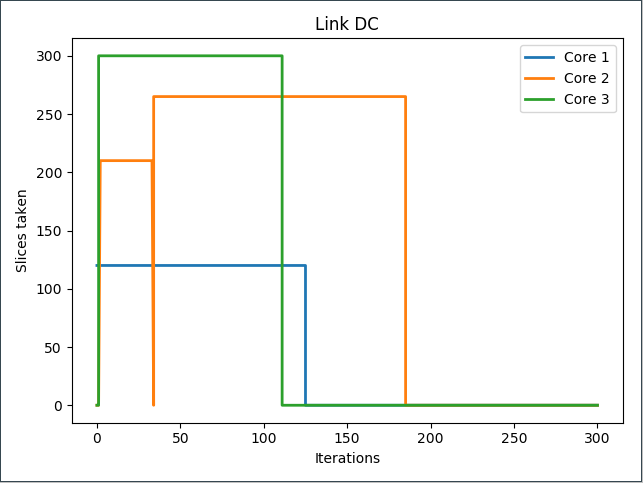
\includegraphics[width=\linewidth]{plot_link.png}
\\
\textbf{Fig. 1} \textit{An example fiber cores allocation for 4 demands}
\end{figure}
\begin{thebibliography}{00}

\bibitem{sdm-walko} P. Lechowicz, K. Walkowiak, M. Klinkowski ``Selection of Spectral-Spatial Channels in SDM
Flexgrid Optical Networks'', Department of Systems and Computer Networks, Wrocław University of Science and Technology, National Institute of Telecommunications, 1 Szachowa Street, 04-894 Warsaw, Poland, 2017

\bibitem{shannon} A.D. Ellis ``The nonlinear Shannon limit and the need for new fibres'', Page 2-3, Tyndall National Institute \& Dept. of Physics, University College Cork, Dyke Parade, Cork, Ireland

\bibitem{flex-intro} D. Rafique, T. Rahman, A Napoli, M. Kuschnerov, G. Lehmann, B. Spinnler ``Flex-grid optical networks: spectrum allocation and nonlinear dynamics of super-channels'', Page 1-2, Coriant R\&D GmbH, St.-Martin-Str. 76, 81541, Munich, Germany, Eindhoven University of Technology, Eindhoven, Netherlands, 2013

\bibitem{sdm-intro} A. Muhammad, G. Zervas, G. Saridis, E. H. Salas, D. Simeonidou, R. Forchheimer ``Flexible and Synthetic SDM Networks with Multi-core-Fibers Implemented by Programmable ROADMs'', Conference: ECOC 2014, At Cannes -France, September 2014

\bibitem{rssa2} D. Siracusa, F. Pederzolli, D. Klonidis, V. Lopez, E. Salvadori ''Resource Allocation Policies in
SDM Optical Networks'',  in Proc. of ONDM, Pisa, Italy, May 2015, pp. 168–173.

\bibitem{walkoartykul} M. Klinkowski, P. Lechowicz, K. Walkowiak ``Survey of Resource Allocation Schemes and Algorithms in Spectrally-Spatially Flexible Optical Networking'', National Institute of Telecommunications, 1 Szachowa Street, 04-894 Warsaw, Department of Systems and Computer Networks, Wrocław University of Science and Technology, Poland, September 2017

\bibitem{wb-box} A. Muhammad, G. Zervas, R. Forchheimer ``Resource Allocation for Space Division Multiplexing: Optical White Box vs. Optical Black Box Networking '', Page 2-3, Linköping University, Linköping, Sweden, High-Performance Networks Group, University of Bristol, UK

\bibitem{rssa} M. Klinkowski, G. Zalewski, K. Walkowiak ``Optimization of Spectrally and Spatially Flexible Optical Networks with Spatial Mode Conversion'', in Proc. of ONDM, Dublin, Ireland, May 2018, pp. 148-153.

\bibitem{python} Python Software Foundation ``Python 3.7.1 documentation'', access via the Internet: \textit{https://docs.python.org/3/} from 16th November 2018.

\bibitem{numpy} The Scipy community ``NumPy Reference'', June 10, 2017, acces via the Internet \textit{https://docs.scipy.org/doc/numpy-1.13.0/reference/} from 16 November 2018

\bibitem{matplotlib} J. Hunter, D. Dale, E. Firing, M. Droettboom ``Matplotlib Release 3.0.0'', September 21, 2018, access via the Internet \textit{https://matplotlib.org/Matplotlib.pdf}


\end{thebibliography}
\vspace{12pt}
\end{document}
